\chapter{Smearing of the Measured Objects}\label{appendix:smear}

As a part of the actions performed for the $t\bar{t}$ kinematic reconstruction, each jet and lepton energy 
and momentum direction is smeared 100 times to have more points where the kinematic equations \ref{alg:LS1}-\ref{alg:LS6} 
are solvable. This means the efficiency of the kinematic reconstruction should increase due to this procedure.
Indeed, the figure \ref{fig:SmearEff} shows that the efficiency applying smearing is higher. However one should also test the
quality of the solutions which are taken from the smeared points.

\begin{figure}[h]
  \centering
  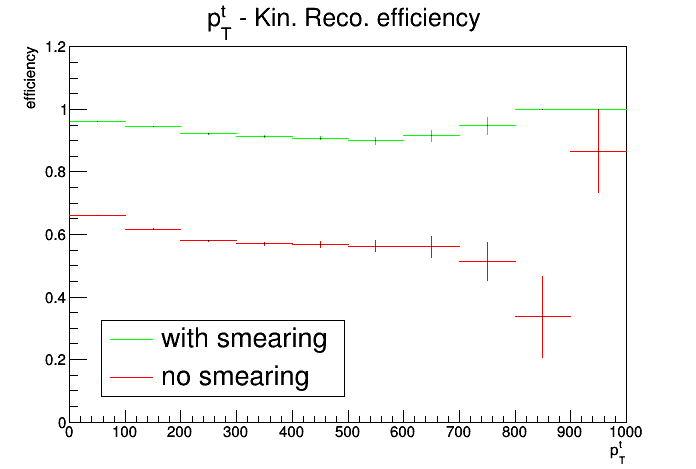
\includegraphics[width=0.8\textwidth]{10_appendices/smearing/Smereff.png}
  \caption{Efficiency of the kinematic reconstruction procedure if the smearing of the reconstructed objects is applied (green)
  and if no smearing is applied (red).}
  \label{fig:SmearEff}
\end{figure}

The figure \ref{fig:RMSsmear} shows the RMS of the solutions which appear only because of smearing compared to the RMS of the
solutions from the central measured values and all smeared solutions. No difference is observed thus the quality of
the smeared solutions is not getting worse.

\begin{figure}[t]
  \centering
  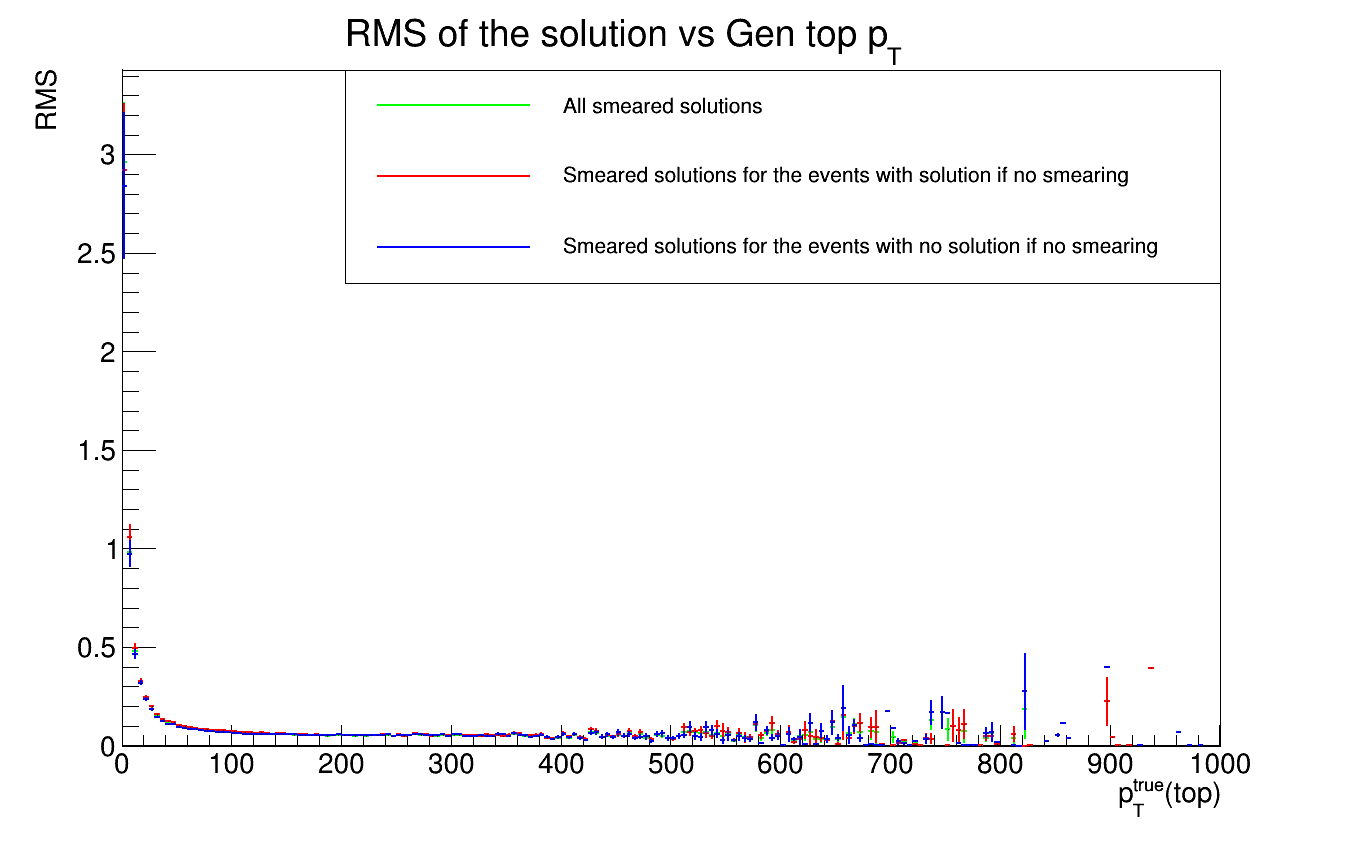
\includegraphics[width=0.8\textwidth]{10_appendices/smearing/RMS.png}
  \caption{RMS of the solutions which appear only due to smearing (blue), smeared solutions which appear in the 
  event even without smearing (red) and all smeared solutions (blue).}
  \label{fig:RMSsmear}
\end{figure}